\subsection{Apresentação do tema}

%SLIDE DE APRESENTAÇÃO DO TEMA
\begin{frame}
    \frametitle{Apresentação do tema}
    \begin{columns}
        \begin{column}{0.5\textwidth}
            \begin{figure}
            \centering
            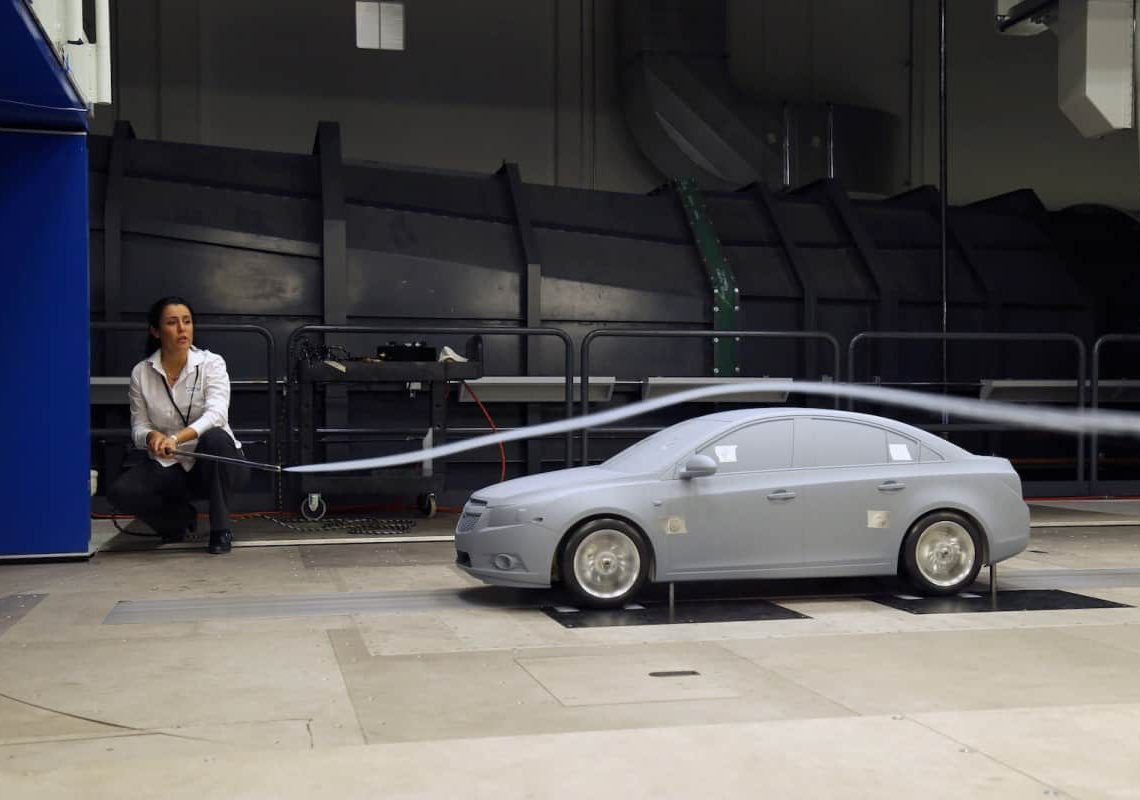
\includegraphics[scale = 0.1]{figuras/tuneltema}
            \end{figure}
        \end{column}
        \begin{column}{0.5\textwidth}
            \begin{figure}
            \centering
            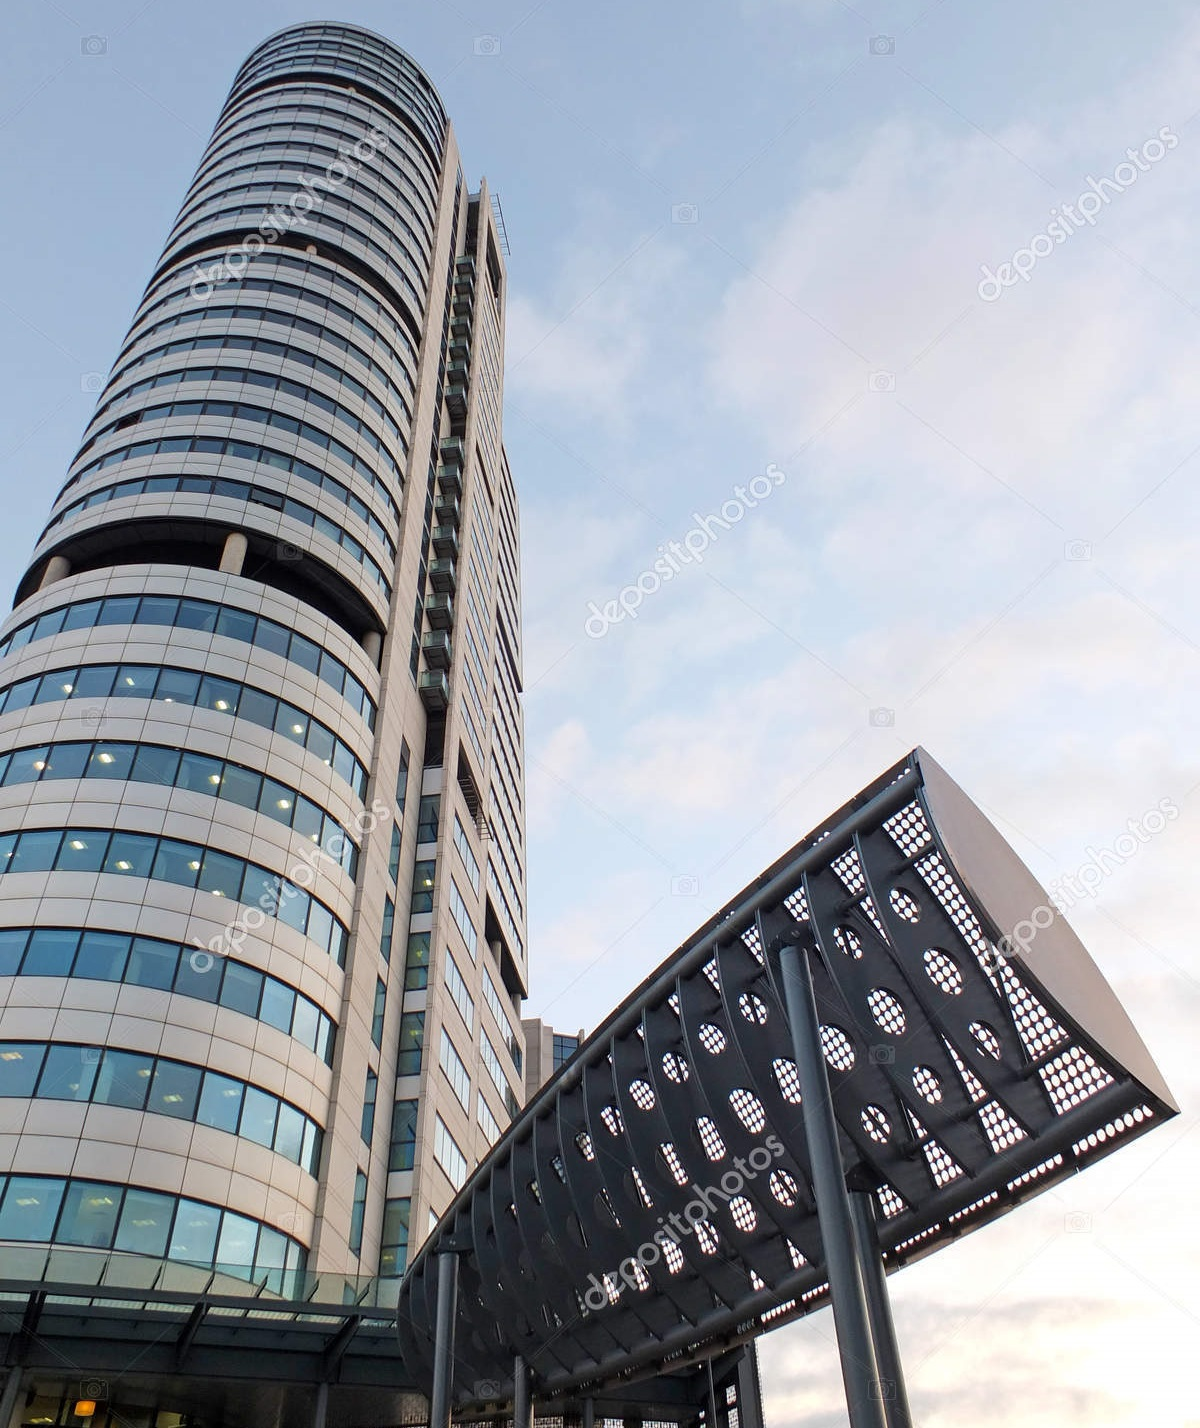
\includegraphics[scale = 0.07]{figuras/edificiotema}
            \caption{Bridgewater Place - Leeds Inglaterra}
            \end{figure}
        \end{column}
    \end{columns}
\end{frame}
    
%\begin{frame}
%\frametitle{Apresentação do tema}
%\begin{itemize}
%    \item A mecânica dos fluidos é uma área muito complexa da engenharia.
%    \item Nem sempre é possível projetar com precisão sem uma análise prévia da ação de esforços sobre algum material. 
%    \item O estudo da ação do ar sobre estruturas pode ser um fator determinante para o sucesso de um projeto. 
%\end{itemize}
%\end{frame}

%SLIDE DE APRESENTAÇÃO DO TEMA
%\begin{frame}
%\frametitle{Apresentação do tema}
%\begin{itemize}
%    \item A análise aerodinâmica pode apresentar dados confiáveis ao projetista para tomada de decisão. 
%    \item Através das leis de similaridade, aplica-se fatores de escala para replicar os resultados em escalas reais. 
%    \item De uma forma menos onerosa é possível se fazer esse estudo em escala reduzida e com condições controladas em laboratório.
%\end{itemize}
%\end{frame}

%SLIDE DE TÚNEL DE VENTO
\begin{frame}
\frametitle{Túnel de vento}

Os túneis de vento são as bancadas de testes para estudos de escoamento de ar, onde é possível simular cenários e avaliar a interação do fluido e estrutura.

\begin{figure}
\centering
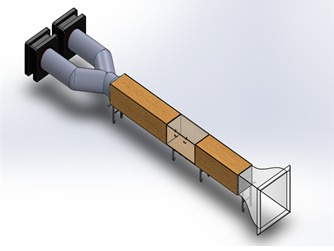
\includegraphics[scale = 0.4]{figuras/tuneldeventosombreado}
\end{figure}

\end{frame}
 
% SLIDE DOS INSTRUMENTOS DE MEDIÇÃO
%\begin{frame}
%\frametitle{Instrumentos de medição}
%
%Uma das grandezas obtidas é a velocidade do fluido, a qual é medida por instrumentos como tubo de Pitot ou sonda de anemômetro de fio quente.
%
%    \begin{columns}
%        \column{0.5\textwidth}
%            \begin{figure}
%            \centering
%            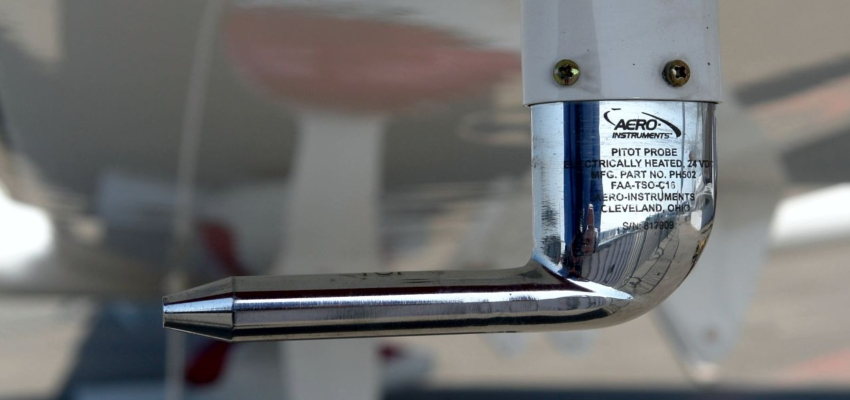
\includegraphics[scale = 0.6]{figuras/tubodepitotaviao}
%            \end{figure}
%        \column{0.5\textwidth}
%            \begin{figure}
%            \centering
%            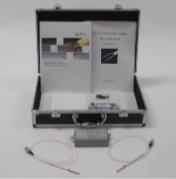
\includegraphics[scale = 0.6]{figuras/sonda}
%            \end{figure}
%    \end{columns}
%\end{frame}

\begin{frame}
\frametitle{Instrumentos de medição}

Uma das grandezas obtidas é a velocidade do fluido, a qual é medida por instrumentos como tubo de Pitot.

    \begin{columns}
        \column{0.5\textwidth}
            \begin{figure}
            \centering
            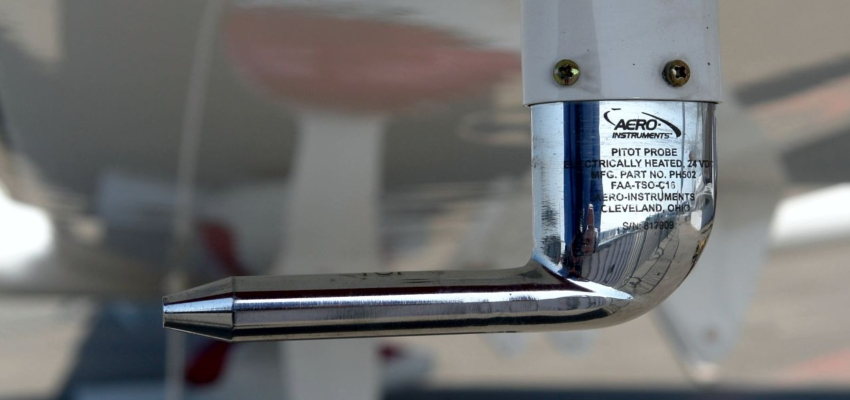
\includegraphics[scale = 0.6]{figuras/tubodepitotaviao}
            \end{figure}
        \column{0.5\textwidth}
            \begin{figure}
            \centering
            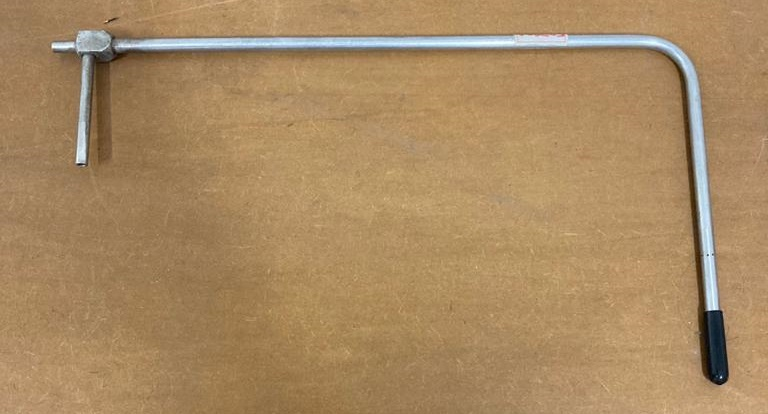
\includegraphics[scale = 0.16]{figuras/tubodepitotlaboratorio}
            \end{figure}
    \end{columns}
\end{frame}
